\centerline{\bf \Huge Дополнительные построения}
\centerline{\bf \Huge }

\begin{flushright}
        \scriptsize{11.11.11. вышел легендарный скайрим.}
\end{flushright}

\problem{1!}
В треугольнике $ABC$ точка $M$ - середина стороны $AC$, точка $P$ лежит на стороне $B C$. Отрезок $AP$ пересекает $BM$ в точке $O$. Оказалось, что $BO=BP$. Найдите отношение $OM: PC$.

\problem{2!}
Докажите равенство треугольников по двум сторонам и медиане, исходящим из одной вершины.

\problem{3}
Прямоугольный лист бумаги перегнули так, как показано на рисунке. Оказалось, что $A C_1=C_1 D$. Найдите отношение $D K: D C$.

\begin{center}
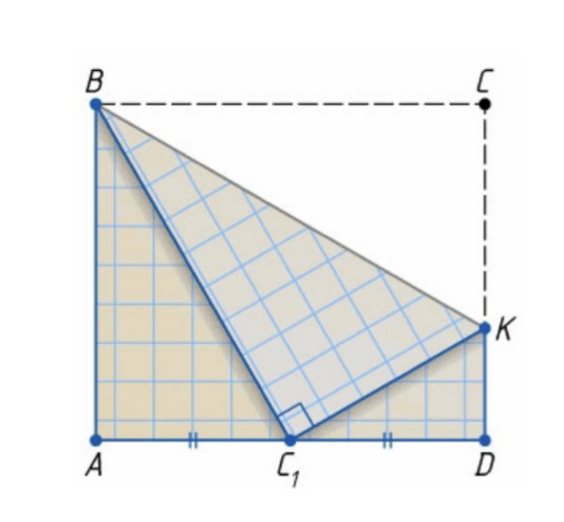
\includegraphics[width=0.4\textwidth]{ЭлМШ 2024-2025/III блок/Киви/HW_Additional_concstructions.png}
\end{center}


\problem{4}
На сторонах $AB$ и $BC$ построены вне его квадраты $ABDE$ и $BCKF$. Доказать, что отрезок $DF$ в 2 раза больше медианы $BP$ треугольника $ABC$.  

\problem{5}
В треугольнике $ABC$ на стороне $AB$ взята точка $P$. Отрезок $CP$ пересекает медиану $BM$ в точке $Q$. Оказалось, что $BP=PQ$ и $BQ=AM$. Найдите угол $AMB$.

